\section{\label{sec:setup:statistical} Experiment design and statistical analysis}

The central theme of this thesis is that we can quantitatively evaluate deeper concepts of understanding by querying humans.
Some natural questions that arise are: how many people should we ask, how much can we trust the quantitative measurements we obtain and does it matter whom we ask or when we ask for feedback?
In this section, we'll cover the basic statistics necessary to answer these questions.

\subsection{What makes for a good evaluation procedure?}

Instead of diving into the abstract criteria that make an evaluation procedure good, let's begin by sketching out the predominant evaluation procedure: \textbf{test collection based evaluation}.
Put simply, a \textbf{test collection} is a set of inputs and expected outputs on which every system is compared.
Each system is assigned a quantitative score based on its performance on the test collection, and different systems are compared on this single quantitative score.
In this subsection, we'll look at how we should construct the test collection, and how the quantitative scores should be computed and compared.

\begin{figure}
  \centering
  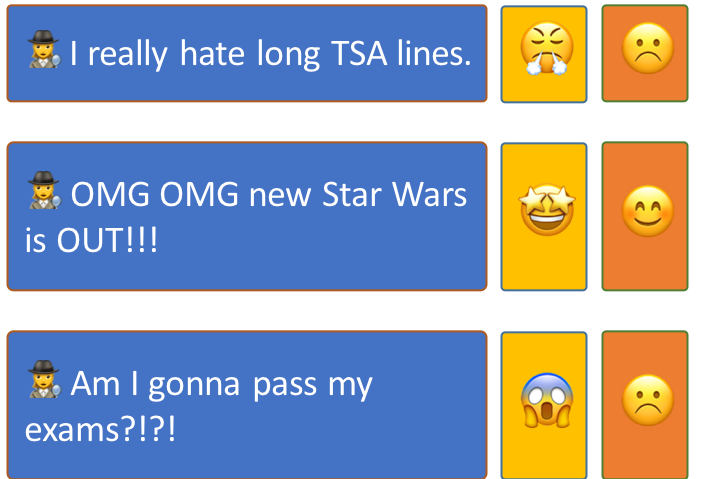
\includegraphics[width=0.8\textwidth]{figures/sentiment-choices}
  \caption[Constructing test collections]{\label{setup:sentiment-choices} \pl{make figure smaller} When constructing a test collection, for example for sentiment classification, one may trade off collecting fine grained labels for more general ones that may be easier or more objective to collect. \pl{explain emoji}}
\end{figure}

\paragraph{Test collections.}
There are many useful ways to define and use a test collection.
Let us take comparing sentiment classification systems as a simple case study (\reffig{setup:stats-overview} \pl{broken}).
Sentiment is inherently multi-faceted (one can express happiness, fear, optimism, etc.) and graded (one can be happy, joyful, ecstatic, etc.), but we may choose to focus simply on distinguishing between positive and negative sentiment because they are more objectively identified by people.
On the other hand, if most systems already distinguish between binary sentiment classes, this evaluation will not be useful in comparing or ranking them.
An additional benefit of simple binary classification is that the test collection can be used to quantitatively measure the quality of the system in question by comparing the system predictions with expected output (e.g., with accuracy).
Unfortunately, this assumption does not hold for the tasks that will be discussed in this thesis: working around this assumption is the key technical contribution of this work. 
However, for the purposes of intuition, we will assume that every output can be perfectly measured \pl{what does measuring an output mean?} using the test collection in this chapter.

Ideally, one would like the test collection to be representative of the inputs that would be found in real life so that the test scores \textbf{faithfully} reflect the systems true performance.
At the same time, we'd like the test collection to be sufficiently large so that we can be confident in the \textbf{reliability} of our conclusions.
Of course, the evaluation designer must weigh these considerations with cost or ease of use.

Next, we will cast the concepts of faithfulness, and reliability into statistical terms.

\begin{figure}
  \centering
  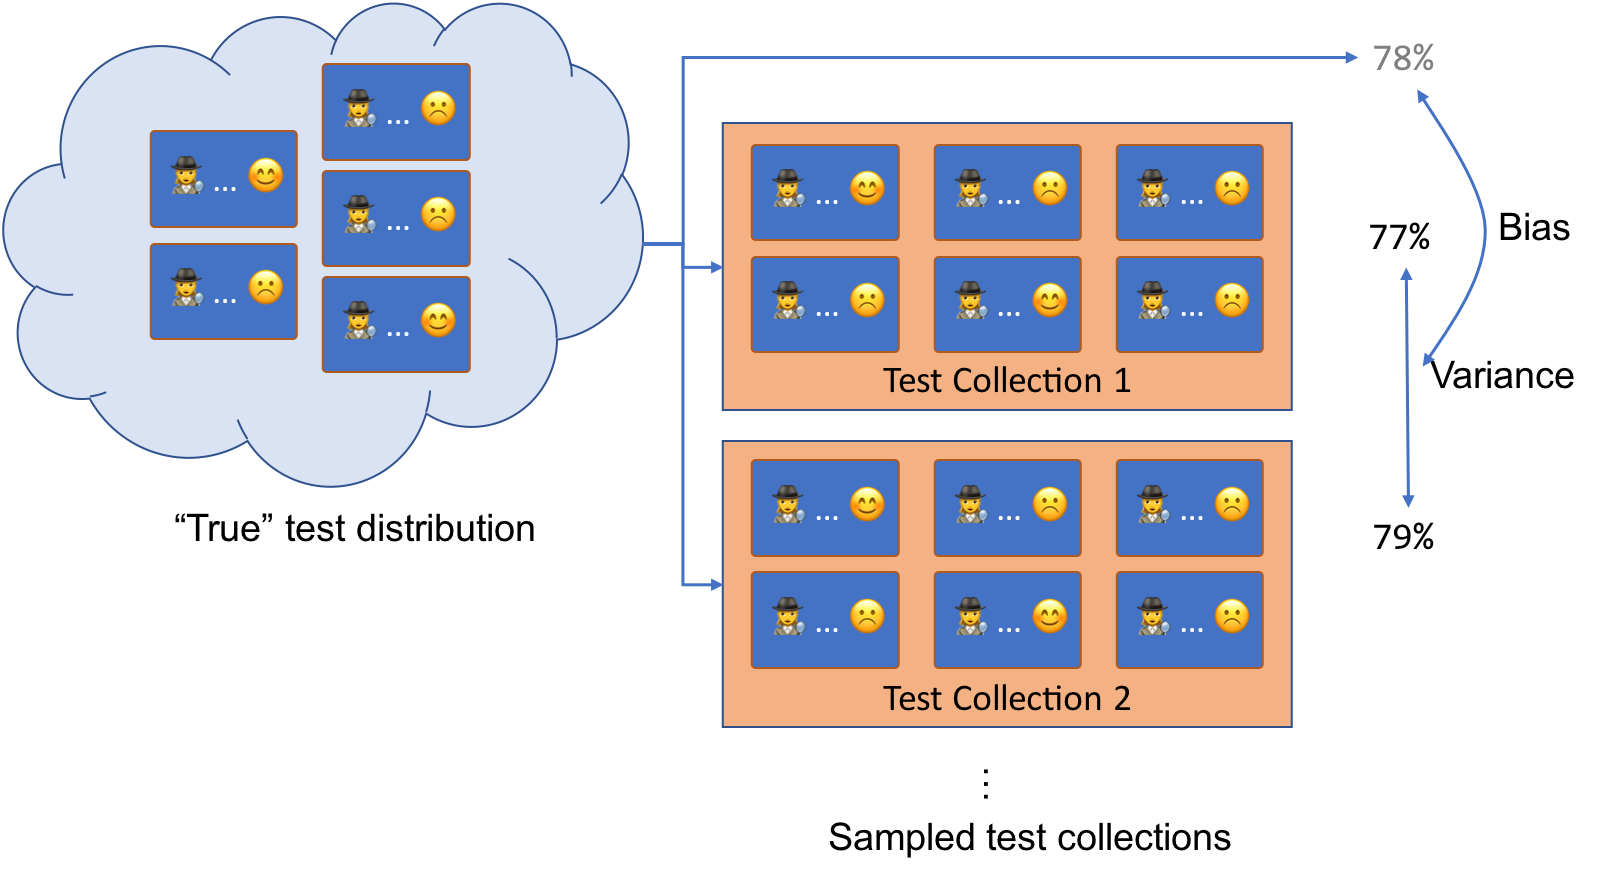
\includegraphics[width=\textwidth]{figures/bias}
  \caption[Bias and variance when evaluating with test collections]{\label{setup:bias} Ideally, a test collection is representative of the true test distribution of examples that occur in the true world.
  When evaluating systems, we would like the performance we measure on our specific test collection to match with what we would get on the true test distribution.
  While the values we measure on any particular test collection may vary, our goal is to eliminate any discrepancy, or bias, between the average over all test collections and the test distribution.
  A good evaluation procedure will have less variance on the performance measure across different test collections.
  }
\end{figure}

\paragraph{Faithfulness as unbiasedness.}
Once we have a test collection $T = \{(x, y)\}$, we can run our systems on it.
An evaluation procedure compares the gold answers $Y$ with the system's predictions $\hat{Y}$.
When does the evaluation procedure \textit{faithfully} measure what it's supposed to?

In this chapter we will assume that given a gold answer $y$ and a system prediction $\yh$, we are can quantitatively measure performance, $f(y, \yh)$.
One example would be accuracy: $f(y, \yh) = 1$ iff $y = \yh$, and $0$ otherwise.
For notational convenience, let $Z = \{(x, y, \yh) \given (x, y) \in T\}$ be the set of system predictions on the test collection and let $f(z)$ be shorthand for $f(y, \yh)$.
\pl{$z$ is not defined; also, $f$ isn't overloaded if $z$ is defined properly; can we make $f$ depend on $x$ too?}

We would like the evaluation procedure to take us from measuring performance on a single example to a more indicative measure of ``average'' performance.
Ideally, we would like to know how well the system works in the ``real world'', i.e., according to some hypothetical test \textit{distribution} of inputs and its corresponding distribution of system predictions $\sP$.
\pl{be more precise what $\sP$ is (the type); in particular, it combines both distribution over $(x,y)$ and $\hat y$; might be good to reify the system $\hat y = S(x)$ or something}
Let the average on this test distribution be $\mu \eqdef \E_{\sP}[f(z)] = \sum_{z \in \sP} f(z)$ \pl{missing normalization}.
We can formalize what it means to be faithful using the concept of unbiasedness: does the evaluation procedure, on average, predict the same measure of performance as $\mu$?

Let $\muh(Z)$ be an estimation algorithm that uses this set to predict $\mu$.
We say that $\muh$ is an \textbf{unbiased estimator} of $\mu$ if
\[
\E_{Z\sim \sP}[\muh(Z)] = \mu,
\]
for any test collection distribution $\sP$. 
One simple method to evaluate $\mu$ on the test collection is to simply take the \textit{average} of system predictions on it:
\[
\muh(Z) = \frac{1}{n} \sum_{z \in Z} f(z).
\]
It is easy to see that $\muh$ is unbiased \textit{if} $T$ was collected in an unbiased manner, e.g.\ through random sampling:
\begin{align*}
  \E_{Z \sim \sP}[\muh(Z)] 
    &= \E_{Z \sim \sP}[\frac{1}{n} \sum_{z \in Z} f(z)] \\
    &= \E_{z \sim \sP}[f(z)] \\
    &= \mu.
\end{align*}

We note that unbiasedness requires our estimators to be unbiased not just on the test collection at hand, but for any hypothetical test collection distribution.
This is a strong condition that seems natural in the context of evaluation: we would like to be able to trust our procedure irrespective of the type of output our systems produce.
At the same time, this condition also presents fundamental limits on the (sample) efficiency of our evaluation procedure, which we will discuss later.

\paragraph{Reliability and variance.}
Unbiasedness alone is not sufficient for a good evaluation procedure: in principle, using a test collection with just a single point would still be unbiased even though its predictions would vary greatly depending on which point was chosen!
Intuitively, the size of our test collection tells us how much \textit{variance} we might expect in our estimate $\muh(Z)$ if we had chosen a different set of test examples.  
We would like our estimate to be indicative of the true performance of our system, as opposed to its performance on just our test collection.
This brings us to the second question we must answer: ``how big should our test collection be in order to \textit{reliably} use our evaluation procedure''?

Suppose that the variance of $f(z)$ when using a \textit{single point} is $\sigma^2_f$, then
elementary statistics~\citep{casella1990statistical} tells us that given test collection with $n$ \textit{independently} drawn samples, the variance of $\muh$, $\Var[\muh] = \frac{\sigma^2_f}{n}$.
Furthermore, if we have sufficiently many examples, then the central limit theorem applies and we can say that with high probability that the true performance estimate $\mu$ will be fairly close to our observed estimate $\muh$
Formally, we have that with probability at least $1 - \delta$,
\begin{align*}
  |\mu - \muh| &\le 2F(\delta) \Std[\muh] \\
  &\le 2F(\delta) \frac{\sigma_f}{\sqrt{n}},
\end{align*}
where $F(\delta)$ is the Gaussian CDF.\@
\pl{Hmm...this is not a precise statement because CLT doesn't hold for any finite $n$, but this looks like a finite sample complexity;
I'd either make it more precise, or just hide things in $O_p(1/\sqrt{n})$
}

This biggest takeaway from this formula is that the \textit{reliability} of our estimate of the true performance $\mu$ is a function not only of the number of samples we have $n$, but also the intrinsic variation of the system's performance \pl{emphasize not just system but underlying data-generating distribution}, $\sigma^2_f$.
When picking a test collection, it is helpful to consider the worse case variance for $\sigma^2_f$; for example, if $f(z)$ is accuracy and only takes the values of $0$ or $1$, the worst case variance is $\frac{1}{4}$.
As a simple rule of thumb, the number of samples we need to be sure with 95\% confidence ($\delta = 0.05$), is about $\frac{1}{\epsilon}^2$ \pl{use parentheses around fraction}: if we want to the true answer to be be within 1\% of the estimate, we fundamentally need about $10,000$ samples.

\subparagraph{Comparing estimation procedures}
The primary way to compare two estimation procedures \pl{replace with 'unbiased estimators'} is to compare their variances: if an estimation procedure is able to combine samples more efficiently than the mean estimator above, we would be able to get equally reliable or precise estimates of performance with fewer samples.
We'll cover when this is possible in the next subsection.

\subparagraph{Practical confidence intervals with the bootstrap}
In practice, we do not actually know what the value of $\sigma^2_f$ is: the best we can do is to compute the sample variance on our test collection, $Z$.
The empirical bootstrap allows us to compute confidence intervals without having to assume any Gaussianity.
The procedure is simple and should be computed whenever performances are reported:
\begin{enumerate}
  \item Suppose we have a test collection $Z$ of size $n$. Let $\muh_0 \eqdef \muh(Z)$ be the estimate on this set.
  \item Construct 1000 to 10000 new test collections $Z^{(i)}$ by drawing $n$ samples from $Z$ \textit{with replacement}.
  \item On each of these collections, evaluate $\muh_{i} \eqdef \muh(Z^{(i)})$ and $\delta_i = \muh_i - \muh_0$
  \item Then the 80\% confidence interval for $\mu$ is $[\muh_0 - \delta_{0.1}, \muh_0 - \delta_{0.9}]$, where $\delta_{0.1}$ and $\delta_{0.9}$ are respectively the 90th percentile and 10th percentile samples of $\delta_i$. 
    \pl{clashing notation in the subscript of $\delta$}
\end{enumerate}

\subsection{Additional considerations}
Now that we've seen the basic definitions of unbiasedness and variance, we will explore some more nuanced statistical concepts:
  Are there fundamental limitations on variance of an estimation procedure?
  Can we measure multiple test distributions with the same set of samples?
  Are there settings in which biased estimation is appropriate? 

\paragraph{Fundamental limitations on the variance of estimators.}
When comparing two estimation procedures \pl{unbiased estimators}, what we are really comparing is their variances.
Fortunately, there are several important theoretical results that provide guarantees on when a particular estimator is optimal, i.e.\ has the least variance among all other estimators.

The first of these results is the \textit{Rao-Blackwell theorem}, which states that any estimator $g(X)$ that depends on data $X$ is strictly improved \pl{varianced reduced} by using sufficient statistics $T(X)$: in other words, $g(T(X))$ will always have equal or less variance than $g(X)$.
Unpacking this statement a bit, given a parameteric \pl{parametrized} distribution $\Pr(x \given \theta)$ that depends on $\theta$, a statistic $t$  computed from the data is \textit{sufficient} if the conditional probability of the data given $t$ does not depend on $\theta$: $\Pr(x \given t, \theta) = \Pr(x \given t)$.
Some popular examples include the mean of a normal distribution with known variance for which the sample mean is a sufficient statistic.
Another way of interpreting sufficiency is that given the sample mean, no more information regarding the normal mean can be obtained from the sample. 
\pl{we're specializing to the mean as opposed to general parameters?}
Rao-Blackwell tells us that the minimum variance estimator for the sample mean \pl{you're estimating the mean, not sample mean} must depend only on the sample mean.
If we would like our estimation procedures to have unbiased guarantees, we must rely on sufficient statistics.
\pl{we were talking about variance, now bias?}

Conveniently, the \textit{Fisher-Neyman factorization theorem} completely characterizes sufficient statistics.
Given a parametric distribution $\Pr(x \given \theta)$, $T$ is a sufficient statistic if and only if non-negative functions $g$ and $h$ can be found such that $\Pr(x \given \theta) = h(x) g_\theta(T(x))$:
  the distribution can be factored into a component that depends only on the data and one that depends on the parameters and the sufficient statistic but not the data as a whole.

Next, we have the \textit{Lehmann-Scheff\'{e} theorem}, which states that any estimator that is unbiased for a given unknown quantity and depends on the data \textit{only} through a \textit{complete sufficient statistic} is the unique best estimator of that quantity in that is has least variance among all other distributions.
Completeness of a statistic is a much stronger condition that requires distinct values of the statistic to correspond to distinct distributions.
Unfortunately, not all distributions or settings have complete statistics, limiting the applicability of Lehmann-Scheff\'{e} and uniformly minimum variance unbiased (UMVU) estimators.

\pl{unclear how these are relevant to our goal of estimating accuracy; try to connect the dots a bit more}

\paragraph{Measuring multiple objectives through importance sampling.}
One of the important criteria for unbiasedness we described in the previous subsection was ensuring that the test collection was sampled in an unbiased manner.
In practice, there are situations in which it is hard to collect a completely random sample or situations in which we would like to use same set of samples to measure multiple objectives, for example the accuracy of a sentiment classification system on a particular subset of documents.
In these situations, importance sampling can be a useful method to ``adjust'' the samples from one distribution to another.

Let $q(z)$ be the distribution under which samples were drawn, and let $p(z)$ be the distribution under which we would like to evaluate $\E_p[f(z)]$.
Given a set of samples $Z$ drawn from $q$, an importance sampling estimator \textit{reweighs} \pl{reweights} each sample from $q$ with the weight $\frac{p(z)}{q(z)}$:
\begin{align}
  \E_q[\frac{p(z)}{q(z)} f(z)] 
  &= \sum_{z \in \sZ} q(z) \frac{p(z)}{q(z)} f(z) \\
  &= \sum_{z \in \sZ} p(z) f(z) \\
  &= \E_p[f(z)].
\end{align}

In order to use importance sampling, we must ensure that $q(z) > 0$ whenever $p(z) > 0$.
Additionally, the closer that $q(z)$ is to $p(z)$, the less variance we will have in our estimate.

\paragraph{Going beyond unbiasedness.}
The main objective of estimators in this thesis is to be unbiased.
While this is a natural and appealing condition for evaluation, it can be too restrictive of a condition and may require too many samples to be practical.
Indeed, it is well known in the statistics literature that there are biased estimators that result in much lower mean square error.
One example of this is the James-Stein estimator, a biased estimator of the mean of Gaussian vectors that has uniformly lower mean squared error than the standard unbiased mean estimator.
Unfortunately, most biased estimators, including the James-Stein estimator, require some prior knowledge of which test distributions are most likely.
When it is reasonable to do so in the evaluation setting, such biased estimators could be considered.
\pl{James-Stein doesn't require any knowledge though to dominate the sample mean; how much it helps of course depends on $\theta^*$}
